\documentclass[12pt,a4paper,titlepage]{article}
\title{Implementazione dell'algoritmo di One-Sided Jacobi Rotation per la decomposizione SVD, tramite librerie NVIDIA CUDA C (codice C) su piattaforma embedded Jetson TK1 (GPU).} 
\author{Matteo Orlandini \& Jacopo Pagliuca}
\date{}

\usepackage[english, italian ]{babel} %the last declared language is the one used in the document
\usepackage[utf8]{inputenc}
\usepackage[T1]{fontenc}
\usepackage{graphicx}
\usepackage{listings}
%inizio impostazioni bibliografia
\usepackage[autostyle,italian=guillemets]{csquotes} 
%autostyle adatta lo stile delle citazioni alla lingua corrente del documento;
%italian=guillemets racchiude automaticamente tra virgolette caporali
%i campi che prevedono le virgolette;
\usepackage[backend=biber, style=numeric, citestyle=numeric,maxcitenames=99,maxbibnames = 99]{biblatex}
%backend=biber dice a biblatex che s’intende usare Biber come motore bibliografico
%style:numeric Anno di pubblicazione: in fondo al riferimento.
%citestyle=numeric Riferimento: numerico ([1], [2], eccetera).
%fine impostazioni bibliografia

\usepackage{float}
\usepackage{hyperref}
\hypersetup{
	bookmarks=true,         % show bookmarks bar?
	unicode=false,          % non-Latin characters in Acrobat’s bookmarks
	pdftoolbar=true,        % show Acrobat’s toolbar?
	pdfmenubar=true,        % show Acrobat’s menu?
	pdffitwindow=false,     % window fit to page when opened
	pdfstartview={FitH},    % fits the width of the page to the window
	%pdftitle={Relazione di Reti di Sensori Wireless per IOT},    % title
	pdfauthor={Matteo Orlandini},     % author
	pdfsubject={Implementazione dell'algoritmo di One-Sided Jacobi Rotation per la decomposizione SVD, tramite librerie NVIDIA CUDA C (codice C) su piattaforma embedded Jetson TK1 (GPU)},   % subject of the document
	pdfcreator={Matteo Orlandini},   % creator of the document
	%pdfproducer={Producer}, % producer of the document
	pdfpagemode={UseOutlines},
	%bookmarksopen,
	pdfstartview={FitH},
	colorlinks=false,       % false: boxed links; true: colored links
	linkcolor={red},
	citecolor={green},
	urlcolor={cyan}
} 

\addbibresource{Bibliografia.bib}

\begin{document}

\begin{titlepage}
	
	\centering
	\includegraphics[width=.2\textwidth]{Immagini/univpmlogo}\par\vspace{1cm}
	{\scshape\LARGE Università Politecnica delle Marche\par}
	\vspace{1cm}
	{\scshape\Large Sistemi Embedded\par}
	\vspace{1.5cm}
	{\huge\bfseries Implementazione dell'algoritmo di One-Sided Jacobi Rotation per la decomposizione SVD, tramite librerie NVIDIA CUDA C (codice C) su piattaforma embedded Jetson TK1 (GPU). \par}
	\vspace{2cm}
	{\Large\itshape Matteo Orlandini \par}
	{\Large\itshape Jacopo Pagliuca\par}
	\vfill
	supervisionato da\par
	Dott. Laura \textsc{Falaschetti} e Prof. Claudio \textsc{Turchetti}
	
	\vfill
	
	% Bottom of the page
	{\large \today\par}
\end{titlepage}

\section{Introduzione}
La seguente tesina descrive il lavoro svolto per la progettazione di un algoritmo di One-sided Jacobi per la decomposizione in valori singolari (SVD) di una matrice, tramite librerie NVIDIA CUDA C. Il codice è stato testato e pensato per un sistema embedded Jetson TK1.

La Jetson TK1 è una scheda embedded realizzato dalla NVIDIA che contiene un processore Tegra K1 SoC nella variante T124. Inoltre essa possiede un sistema operativo Ubuntu Linux. La versione di CUDA presente nel dispositivo era la 6.5, la quale ha limitato alcune scelte progettuali in quanto non consente la chiamata di kernel all'interno di altri kernel.

In facoltà era già stato sviluppato un codice in C per la SVD ottimizzato per lavorare su CPU. Il nostro lavoro era quello di confrontare i nostri risultati con quelli precedentemente ottenuti e valutare la possibilità di una implementazione alternativa che sfruttasse appieno le potenzialità della GPU della Jetson.

Come base per il nostro lavoro abbiamo studiato il linguaggio di programmazione e l'architetttura CUDA tramite \cite{Cheng:ProfessionalCudaProgramming} e \cite{Sanders:CudaByExample}. In seguito sono stati analizzati diversi articoli che descrivevano vari approcci per l'ottimizzazione dell'algoritmo su GPU, per poi realizzare la nostra versione, i cui risultati sono molto simili a quelli ottenuti negli articoli.

Per lavorare sulla scheda abbiamo sfruttato il protocollo SSH dal dipartimento, in modo da poter connettersi alla scheda senza la necessità di spostarla. Alla fine della realizzazione del progetto non è però stato possibile accedere al dipartimento e quindi ai risultati esatti del tempo computazionale che necessita l'algoritmo. Abbiamo quindi usato come riferimento una NVIDIA GTX 610M, i cui risultati erano proporzionali a quelli ottenuti con la Jetson, anche se differenti.

\subsection{SVD}
In algebra lineare, la decomposizione ai valori singolari (SVD), è una fattorizzazione di una matrice in tre diverse matrici basata sull'uso di autovalori e autovettori.

La decomposizione di una matrice $\mathbf{A}$ si basa sul \textit{teorema fondamentale dell'algebra lineare}: 

Data una matrice $\mathbf{A}\in\mathbb{C}^{m\times n}$ di rango $\rho$, la decomposizione in valori singolari di $\mathbf{A}$ è rappresentata dal prodotto di due matrici unitarie $\mathbf{U}\in\mathbb{C}^{m\times m}$, $\mathbf{V}\in\mathbb{C}^{n\times n}$ e una matrice diagonale $\mathbf{\Sigma}\in\mathbb{R}^{m\times n}$, come mostrato in (\ref{svd}).
\begin{equation}\label{svd}
\mathbf{A}=\mathbf{U}\mathbf{\Sigma}\mathbf{V}^H
\end{equation}
Le colonne di $\mathbf{U}$ sono chiamate \textit{vettori singolari sinistri} di $\mathbf{A}$ mentre le colonne di $\mathbf{V}$ sono i \textit{vettori singolari destri} di $\mathbf{A}$. Inoltre, $\mathbf{\Sigma}$ è una matrice reale non negativa del tipo
\[
\mathbf{\Sigma}=\begin{bmatrix}
\sigma_1 & 0 & 0 & 0\\
0 & \ddots & 0 & 0\\
0 & 0 & \sigma_{\rho} & 0\\
0 & 0 & 0 & 0
\end{bmatrix}
\]
Gli elementi diagonali di $\mathbf{\Sigma}$ sono i \textit{valori singolari} di $\mathbf{A}$ e sono solitamente in ordine decrescente: $\sigma_1 \geq \sigma_2 \geq ... \geq \sigma_{\rho} > 0, \sigma_{\rho+1}=...=0$.

Nel caso in cui $\mathbf{A}\in\mathbb{R}^{m\times n}$ l'equazione (\ref{svd}) diventa:
\begin{equation}\label{svd2}
\mathbf{A}=\mathbf{U}\mathbf{\Sigma}\mathbf{V}^T
\end{equation}
dove $\mathbf{U}\in\mathbb{R}^{m\times m}$ e $\mathbf{V}\in\mathbb{R}^{n\times n}$ sono matrici ortonormali.
\begin{eqnarray}
\mathbf{U}\mathbf{U}^T=\mathbf{U}^T\mathbf{U}=I^{m\times m}\\
\mathbf{V}\mathbf{V}^T=\mathbf{V}^T\mathbf{V}=I^{n\times n}
\end{eqnarray}
Unendo queste due proprietà all'equazione (\ref{svd2}) si possono ricavare l'espressione di $\mathbf{A}\mathbf{A}^T$:
\[
\mathbf{A}\mathbf{A}^T=\mathbf{U}\mathbf{\Sigma}\mathbf{V}^T(\mathbf{U}\mathbf{\Sigma}\mathbf{V}^T)^T=\mathbf{U}\mathbf{\Sigma}\mathbf{V}^T\mathbf{V}\mathbf{\Sigma}\mathbf{U}^T=\mathbf{U}\mathbf{\Sigma}^2\mathbf{U}^T
\]
Allo stesso modo, per $\mathbf{A}^T\mathbf{A}$:
\[
\mathbf{A}^T\mathbf{A}=\mathbf{V}\mathbf{\Sigma}^2\mathbf{V}^T
\]
La SVD ha numerose applicazioni nel campo dell'algebra lineare. Innanzitutto fornisce delle informazioni importanti sulla matrice $\mathbf{A}$, come il suo rango, qual è il suo nucleo e qual è la sua immagine. Viene usata per definire la pseudo-inversa di una matrice rettangolare utile per la risoluzione del problema dei minimi quadrati. Trova utilizzo anche nella risoluzione di sistema di equazioni lineari omogeneo.

Un'altra importante applicazione riguarda l'approssimazione della matrice $\mathbf{A}$, con una di rango inferiore (SVD troncata), utilizzata nell'elaborazione di immagini e nell'elaborazione dei segnali.

La SVD ha anche note applicazioni nel campo dell'analisi delle componenti principali.




\subsection{One Sided Jacobi SVD}
One Sided Jacobi SVD: spiegazione dell'algoritmo

\subsection{CUDA}
CUDA: spiegazione del funzionamento della GPU (vedere Professional CUDA C Programming e Cuda by Example)

\newpage
\section{Sequential implementation}
%Descrizione algoritmo sequential
%Dal capitolo Jacobi rotation nell'articolo Acosta
%https://tex.stackexchange.com/questions/55054/bordermatrix-with-brackets-instead-of-parentheses
\makeatletter
\def\bbordermatrix#1{\begingroup \m@th
	\global\let\perhaps@scriptstyle\scriptstyle
	\@tempdima 4.75\p@
	\setbox\z@\vbox{%
		\def\cr{%
			\crcr
			\noalign{%
				\kern2\p@
				\global\let\cr\endline
				\global\let\perhaps@scriptstyle\relax
			}%
		}%
		\ialign{$\make@scriptstyle{##}$\hfil\kern2\p@\kern\@tempdima
			&\thinspace\hfil$\perhaps@scriptstyle##$\hfil
			&&\quad\hfil$\perhaps@scriptstyle##$\hfil\crcr
			\omit\strut\hfil\crcr
			\noalign{\kern-\baselineskip}%
			#1\crcr\omit\strut\cr}}%
	\setbox\tw@\vbox{\unvcopy\z@\global\setbox\@ne\lastbox}%
	\setbox\tw@\hbox{\unhbox\@ne\unskip\global\setbox\@ne\lastbox}%
	\setbox\tw@\hbox{$\kern\wd\@ne\kern-\@tempdima\left[\kern-\wd\@ne
		\global\setbox\@ne\vbox{\box\@ne\kern2\p@}%
		\vcenter{\kern-\ht\@ne\unvbox\z@\kern-\baselineskip}\,\right]$}%
	\null\;\vbox{\kern\ht\@ne\box\tw@}\endgroup}
\def\make@scriptstyle#1{\vcenter{\hbox{$\scriptstyle#1$}}}
\makeatother

La rotazione di Jacobi è una rotazione di un sottospazio bidimensionale in uno spazio $n$-dimensionale, denotato da \textbf{J}. Dopo l'applicazione di questa trasformazione, una coppia di elementi di una matrice simmetrica  $\mathbf{B} \in \mathbb{R}^{n \times n}$ sono azzerati, come indicato in $\mathbf{B} \longmapsto \mathbf{J^TBJ} = \mathbf{B}'$ dove $c = \cos (\theta)$, $s = \sin (\theta)$ e $\theta$ è l'angolo di rotazione nel piano $(i, j)$. Solo le righe $i$-esima e $j$-esima di $\mathbf{B}$ sono interessate. In modo simile, solo le colonne $j$-esima e $i$-esima sono interessate. Gli elementi $b'_{ij}$, $b'_{ji}$,  $b'_{ii}$ e $b'_{jj}$ in $\mathbf{B}$ vengono utilizzati per calcolare gli angoli nelle matrici di rotazione che eliminano gli elementi $b'_{ij}$ e $b'_{ji}$ come mostrato in Eq.~\ref{eq:J_matrix}. 
\begin{equation} \label{eq:J_matrix}
%
\mathbf{J}(i,j,\theta) = \bbordermatrix{
	& & & i& &j &  & \cr
	&1 & \dots & 0 & \dots & 0 &\dots & 0 \cr
	&\vdots & \ddots & \vdots & & \vdots & & \vdots\cr
	i&0 & \dots & c & \dots & s & \dots & 0 \cr
	&\vdots & & \vdots & & \vdots & & \vdots\cr
	j&0 & \dots & -s & \dots & c & \dots & 0\cr
	&\vdots & & \vdots & & \vdots & \ddots & \vdots\cr
	&0 & \dots & 0 & \dots & 0 & \dots & 1\cr
}
%
\end{equation}
L'algoritmo Jacobi esegue una sequenza di aggiornamenti della matrice $\mathbf{B}$ che viene ortogonalizzata, ogni nuova matrice $\mathbf{B}$ è più diagonale rispetto alla predecedente.  Quando gli elementi fuori della diagonale sono abbastanza piccoli, possono essere considerati nulli. In particolare, ogni rotazione Jacobi comporta una pre-moltiplicazione e una post-moltiplicazione di $\mathbf{B}$ per matrici ortogonali. In generale, vengono eseguite $(n^2 - n)/2$ rotazioni (nel caso di una matrice simmetrica) cercando di rendere zero tutti gli elementi fuori diagonale. Queste $(n^2 - n)/2$ transformazioni costituiscono una scansione (sweep). Comunemente, le rotazioni di Jacobi vengono applicate utilizzando uno dei seguenti approcci: esecuzione di rotazioni cicliche per riga o per colonna. In questi approcci, la coppia $(i, j)$ è selezionata riga per riga o colonna per colonna, rispettivamente. Ad esempio, se $n = 4$, la sequenza di rotazione è: $(i, j) = (1,2), (1,3), (1,4), (2, 3), (2,4), (3,4)$.
\cite{Acosta:SVD}

\newpage
\section{Parallel implementation}
%Descrizione algoritmo parallel
%Dal capitolo PARALLELIZING THE ONE-SIDED JACOBI nell'articolo Romer
Parallelizzare la One-Sided Jacobi implica il partizionamento di $n(n-1)/2$ coppie di colonne che devono essere ortogonali a ciascuna scansione (sweep) in gruppi di coppie di colonne indipendenti. Ogni sweep viene quindi elaborato un set alla volta, ortogonalizzando in parallelo le coppie di colonne all'interno del set corrente.

Le coppie di colonne per ciascun set vengono generate utilizzando un algoritmo di pianificazione round-robin. Concettualmente, ogni round rappresenta un set e gli abbinamenti all'interno di un round corrispondono agli abbinamenti di colonne all'interno di quel set. Ad esempio, di seguito sono riportati tutti i possibili set contenenti le rispettive coppie di colonne per $n = 6$:
\begin{center}
	Set 1 = $\{(1,2),(3,4),(5,6)\}$\\
	Set 2 = $\{(1,4),(2,6),(3,5)\}$\\
	Set 3 = $\{(1,6),(2,3),(4,5)\}$\\
	Set 4 = $\{(1,5),(2,4),(3,6)\}$\\
	Set 5 = $\{(1,3),(2,5),(4,6)\}$\\
\end{center}
In generale, ogni set contiene $\hat{n}/2$ coppie di colonne ortogonalizzate in parallelo, dove $\hat{n}$ è il prossimo numero intero pari maggiore o uguale a $n$. Se $n$ è dispari, quindi ogni set avrà una colonna accoppiata con una colonna "fantasma"; le coppie che contengono la colonna fantasma non sono ortogonali. In base a questo schema, sono necessari $\hat{n}/2 - 1$ set per completare una sweep completa.

La coppia di colonne $(p', q')$ ortogonalizzata dalla $i-$esima rotazione in un set viene calcolata direttamente dalla coppia di colonne $(p, q)$ corrispondente ortogonalizzata dalla $i-$esima rotazione nel set precedente. In pratica, questo schema è più adatto per l'esecuzione su una GPU in cui la larghezza di banda di calcolo supera notevolmente la larghezza di banda di memoria. \cite{Romer:SVD}

%Dal capitolo Parallel-Order Jacobi algorithm nell'articolo Acosta
Nelle tradizionali implementazioni sequenziali dell'algoritmo Jacobi, il parallelismo non viene sfruttato, principalmente a causa della dipendenza dei dati di una rotazione con la sua precedente. L'algoritmo Jacobi parallelo sfrutta il massimo parallelismo per la decomposizione di una matrice simmetrica. Questo algoritmo richiede un numero di step pari a $n - 1$, in cui in ogni step si compiono $n/2$ rotazioni. Tutte le rotazioni all'interno di uno step possono essere eseguite in parallelo. \cite{Acosta:SVD}

%Dal capitolo IMPLEMENTING THE SVD USING CUDA nell'articolo Romer
Si è usato CUDA per implementare una SVD parallela basata sul metodo One-Sided Jacobi descritto in~\ref{sec:OneSidedJacobi}. La matrice di input $A \quad (m \times n)$ è una matrice reale in cui $m \geq n$. Se $m < n$, la SVD di A può essere calcolata dalla SVD di $A^T = V \Sigma U^T$. Le matrici di input sono salvate in column-major order e single-precision floating point. \cite{Romer:SVD}

Viene ora mostrata l'implementazione in CUDA dell'algoritmo parallel. Il codice che richiama il kernel che esegue l'algoritmo One-Sided Jacobi parallel è il seguente.
\begin{lstlisting}
while(!host_exit_flag) {
	++iter;
	host_exit_flag = true; 
	cudaMemcpy(dev_exit_flag, &host_exit_flag, sizeof(bool), cudaMemcpyHostToDevice);
	for(int set = 0; set < cols; set++) {
		scheduling<<<1, 1>>> (dev_v1, dev_v2, cols);
		round <<<cols/2, rows>>> (dev_B, dev_v1, dev_v2, cols, rows, dev_exit_flag);		
	}
	cudaMemcpy( &host_exit_flag, dev_exit_flag, sizeof(bool), cudaMemcpyDeviceToHost);
}
\end{lstlisting}
Le variabili \textit{host\_exit\_flag}, \textit{iter} e \textit{B} svolgono le stesse funzioni descritte nel codice~\ref{code:while_loop}.

La variabile \textit{set} contiene............

I vettori \textit{v1} e  \textit{v2} servono a........

Il kernel \textit{scheduling} serve a........ ed è definito come segue
\begin{lstlisting}
__global__ void scheduling (int *v1, int *v2, int cols){
	int tmp = v2[0];
	for (int i = 0; i < (cols/2) - 1; i++)
	v2[i] = v2[i+1];	
	v2[cols/2 - 1] = v1[cols/2 - 1];
	for (int i = (cols/2) -1; i > 1; i--)
	v1[i] = v1[i-1];	
	v1[1] = tmp;
}
\end{lstlisting}

Il kernel \textit{round} chiama un numero di blocchi pari alla metà del numero delle colonne della matrice e un numero di thread pari alle righe della matrice perché......... Questo kernel esegue............

Nei capitoli~\ref{sec:Global},~\ref{sec:Semi_Shared} e~\ref{sec:Shared} sono presentate tre varianti del kernel \textit{round} a seconda della memoria in cui viene immagazzinata la matrice \textit{B}.

Il calcolo dei valori singolari è eseguito dal kernel~\textit{computeSingVals}, codice~\ref{code:computeSingVals}, precedentemente descritto.

\subsection{Global Memory}
%Descrizione algoritmo Global Memory
\label{sec:Global}
In questo capitolo viene mostrato il kernel \textit{round} che usa la global memory.
\begin{lstlisting}
__global__ void round (float *B, int *v1, int *v2, int cols, int rows, bool * exit_flag) {
	int blockId = blockIdx.x; //max(blockId) = (cols/2) - 1
	int threadId = threadIdx.x; //max(blockId) = rows - 1
	__shared__ float alpha, beta, gamm;
	if ((blockId < cols/2) && (threadId < rows)){
		int i = *(v1 + blockId);
		int j = *(v2 + blockId);
		float * pi = B + rows * i + threadId;
		float * pj = B + rows * j + threadId;
		alpha = beta = gamm = 0;
		__syncthreads();
		atomicAdd(&alpha, *pi * *pi);
		atomicAdd(&beta, *pj * *pj);	
		atomicAdd(&gamm, *pi * *pj);
		__syncthreads();
		if (*exit_flag) {
			const float limit = fabsf(gamm) / sqrtf(alpha * beta);
			if (limit > eps){
				*exit_flag = false;
			}
		} 
		const float tao = (beta - alpha) / (2 * gamm);
		const float t = sign (tao) / (fabsf(tao) + sqrtf(1 + tao * tao)); 
		const float c = expf(-0.5f * log1pf(t * t));
		const float s = c * t;
		const float tmp = *pi;
		*pi = c * tmp - s * *pj;
		*pj = s * tmp + c * *pj;
	}
}
\end{lstlisting}

\subsection{Semi Shared Memory}
%Descrizione algoritmo Semi Shared Memory
\label{sec:Semi_Shared}
In questa implementazione le variabili \textit{alpha}, \textit{beta}, \textit{gamm}, \textit{limit}, \textit{tao}, \textit{t}, \textit{c}, \textit{s}, \textit{i} e \textit{j} sono contenute nella shared memory e sono identificate dall'attributo \textit{\_\_shared}. I puntatori \textit{pi} e \textit{pj} che contengono l'indirizzo di memoria degli elementi della coppia di vettori colonna i-esimo e j-esimo non sono contenuti invece contenuti nella shared memory.
\begin{lstlisting}
__global__ void round (float *B, int *v1, int *v2, int cols, int rows, bool * exit_flag) {
	int blockId = blockIdx.x; //max(blockId) = (cols/2) - 1
	int threadId = threadIdx.x; //max(blockId) = rows - 1
	float * pi, *pj;
	__shared__ float alpha, beta, gamm, limit, tao, t, c, s;
	__shared__ int i, j;
	if ((blockId < cols/2) && (threadId < rows)){
		i = *(v1 + blockId);
		j = *(v2 + blockId);
		pi = B + rows * i + threadId;
		pj = B + rows * j + threadId;
		alpha = beta = gamm = 0;
		__syncthreads();
		atomicAdd(&alpha, *pi * *pi);
		atomicAdd(&beta, *pj * *pj);	
		atomicAdd(&gamm, *pi * *pj);
		__syncthreads();
		if ( *exit_flag) {
			limit = fabsf(gamm) / sqrtf(alpha * beta);
			if (limit > eps){
				*exit_flag = false;
			}
		} 
		tao = (beta - alpha) / (2 * gamm);
		t = sign (tao) / (fabsf(tao) + sqrtf(1 + tao * tao)); 
		c = expf(-0.5f * log1pf(t * t));
		s = c * t;
		const float tmp = *pi;
		*pi = c * tmp - s * *pj;
		*pj = s * tmp + c * *pj;
	}
}
\end{lstlisting}	

\subsection{Shared Memory}
%Descrizione algoritmo Shared Memory
\label{sec:Shared}
Nell'implementazione in cui viene usata la shared memory per lavorare con la matrice \textit{B} si può notare che tra le parentesi angolari che indicano i blocchi e i thread allocati per il kernel è presente una terza variabile come si può vedere nel codice seguente
\begin{lstlisting}
round <<<cols/2, rows, 2*rows*sizeof(float)>>> (dev_B, dev_v1, dev_v2, cols, rows, dev_exit_flag);
\end{lstlisting}
Questo permette di allocare dinamicamente la memoria shared, che può essere utilizzata quando la quantità di memoria condivisa non è nota al momento della compilazione. In questo caso, la dimensione di allocazione della memoria shared per ogni blocco deve essere specificata (in byte) utilizzando un terzo parametro di configurazione come mostrato precedentemente.

La memoria allocata corrisponde a \textit{2*rows*sizeof(float)} in quando ad ogni blocco viene assegnata una coppia di colonne. Ogni thread lavora su due elementi della coppia opportuna appartenenti alla riga corrispondente al thread.
Mentre in precedenza le due colonne venivano modificate tramite puntatori, in questo caso vengono copiate nella memoria shared che richiede minor tempo di accesso per la lettura e la scrittura. La rotazione delle colonne viene quindi fatta internamente ad ogni blocco per poi trasferire di nuovo la variabile \textit{arr} in global, aggiornando la matrice originale.
\begin{lstlisting}
__global__ void round (float *B, int *v1, int *v2, int cols, int rows, bool * exit_flag) {
	int blockId = blockIdx.x;
	int threadId = threadIdx.x;
	__shared__ float alpha, beta, gamm, limit, tao, t, c, s, tmp;
	extern __shared__ float arr[];
	__shared__ int i, j;
	if ((blockId < cols/2) && (threadId < rows)){
		i = *(v1 + blockId);
		j = *(v2 + blockId);
		arr[threadId] = *(B + rows * i + threadId);
		arr[threadId+rows] = *(B + rows * j + threadId);
		alpha = beta = gamm = 0;
		__syncthreads();
		atomicAdd(&alpha, arr[threadId] * arr[threadId]);
		atomicAdd(&beta, arr[threadId+rows] * arr[threadId+rows]);	
		atomicAdd(&gamm, arr[threadId] * arr[threadId+rows]);
		__syncthreads();
		if (*exit_flag) {
			limit = fabsf(gamm) / sqrtf(alpha * beta);
			if (limit > eps){
				*exit_flag = false;
			}
		}
		tao = (beta - alpha) / (2 * gamm);
		t = sign (tao) / (fabsf(tao) + sqrtf(1 + tao * tao)); 
		c = expf(-0.5f * log1pf(t * t));
		s = c * t;
		tmp = arr[threadId];
		arr[threadId] = c * tmp - s * arr[threadId+rows];
		arr[threadId+rows] = s * tmp + c * arr[threadId+rows];
		*(B + rows * i + threadId) = arr[threadId];
		*(B + rows * j + threadId) = arr[threadId+rows];
	}
}
\end{lstlisting}
Il kernel con memoria shared dinamica, \textit{round}, dichiara l'array nella shared memory utilizzando un array extern senza dimensione(si noti le parentesi vuote e l'uso dell'identificatore \textit{extern}). La dimensione è implicitamente determinata dal terzo parametro di configurazione all'avvio del kernel.
\begin{lstlisting}
extern __shared__ float arr[];
\end{lstlisting}

\newpage
\section{Performance}
\label{sec:Performance}
Per testare gli algoritmi presentati nei capitoli~\ref{sec:Sequential},~\ref{sec:Global},~\ref{sec:Semi_Shared} e~\ref{sec:Shared} sono state usate 6 matrici generate con Matlab tramite la funzione \textit{rand} che restituisce un numero random distribuito uniformemente nell'intervallo $(0,1)$. Queste matrici hanno un aspect ratio, cioè il rapporto tra la larghezza (colonne) e l'altezza di una matrice, di $4:3$. Le matrici generate hanno 32, 48, 96, 128, 160 e 200 righe. 

I grafici presentati in questo capitolo sono stati generati usando un pc con CPU Intel i7-3630 QM @2.40 GHz, 8GB di RAM e una GPU NVIDIA Geforce GTX 610M poiché non era possibile usare la scheda JETSON per produrre i risultati.

I grafici~\ref{fig:Mean_Square_Error} e~\ref{fig:Mean_Square_Error_Zoom} mostrano come cambia l'errore quadratico medio dei valori singolari calcolati al variare dell'algoritmo One-Sided Jacobi usato e del numero di colonne della matrice usata. Il MSE è calcolato come 
$$ \text{MSE} = \dfrac{1}{n} \sum_{i = 1}^{n} (Y_i - \hat{Y}_i)^2$$
dove $n$ è il numero di colonne della matrice, $Y$ è il vettore che contiene i valori singolari calcolati dalla funzione \textit{svd} di Matlab e $\hat{Y}$ è l'array \text{AUX1}, mostrato nel codice~\ref{code:computeSingVals}, che contiene i valori singolari calcolati dalla GPU. Nel grafico~\ref{fig:Mean_Square_Error} si può vedere che l'errore quadratico massimo è $10^{-4}$, coerente con la variabile \textit{eps} posta pari a questo valore nel codice~\ref{code:eps}. La figura~\ref{fig:Mean_Square_Error_Zoom} mostra che per tutte le matrici con meno di 150 colonne l'errore quadratico medio si mantiene nell'intorno di $10^{-9}$.
\begin{figure}[H]
	\centering
	\subfloat[][Errore quadratico medio]
	{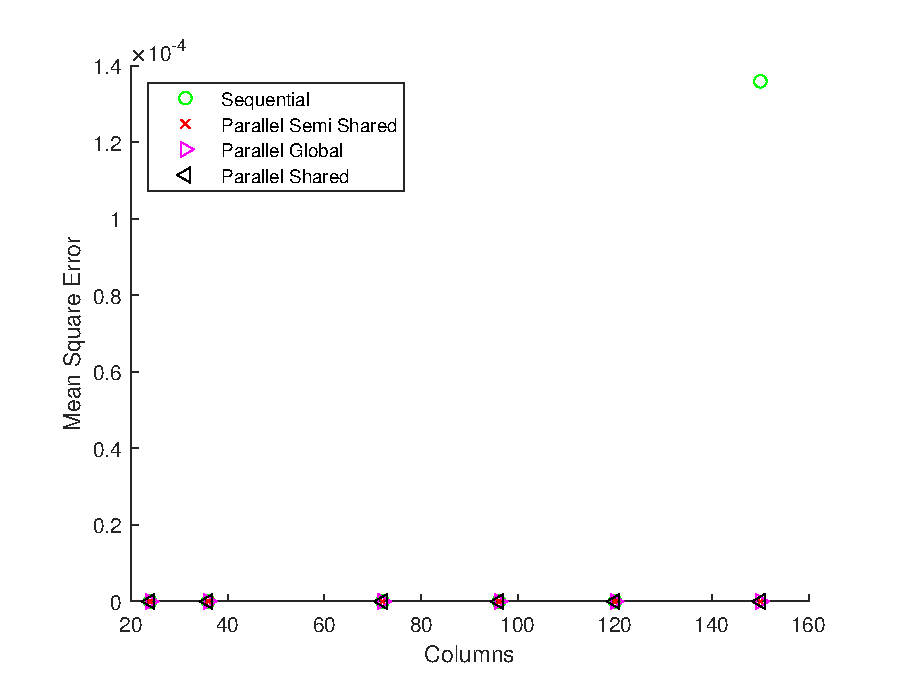
\includegraphics[width=.6\textwidth]{Grafici/Mean_Square_Error.eps} \label{fig:Mean_Square_Error}}
	\subfloat[][Dettaglio dell'errore quadratico medio]
	{\includegraphics[width=.6\textwidth]{Grafici/Mean_Square_Error_Zoom.eps} \label{fig:Mean_Square_Error_Zoom}} \\
	\caption{Confronto dell'errore quadratico medio}
\end{figure}
I grafici che seguono sono stati ottenuti usando la funzione \textit{cudaEventRecord} che registra un evento. Questa funzione permette di gestire due \textit{event}, chiamati \textit{start} e \textit{stop}, e di misurare il tempo intercorso tra i due. \textit{Start} viene registrato prima del ciclo \textit{while} presentato nel codice~\ref{code:sequential_loop}, mentre \textit{stop} quando si esce da questo loop. Dato che nel ciclo si esegue la One Sided Jacobi rotation si misura il tempo trascorso tra l'entrata e l'uscita del ciclo.

Le figure~\ref{fig:ColumnsTime} e~\ref{fig:ColumnsTime_Zoom} mostrano come cambia il tempo di esecuzione dell'algoritmo One-Sided Jacobi al variare della grandezza della matrice, in particolare del numero di colonne in quanto tutte le matrici di prova hanno lo stesso aspect ratio. L'algoritmo più veloce rimane quello che viene eseguito sull'host, mentre tra gli algoritmi testati sul device il migliore in termini di tempo è quello parallelo che usa la memoria shared. Questo è inoltre confermato dal fatto che questa è la memoria più veloce e può arrivare ad essere fino a 100 volte più veloce della memoria global. \cite{Cheng:ProfessionalCudaProgramming} \cite{Sanders:CudaByExample}
\begin{figure}[H]
	\centering
	\subfloat[][Relazione tra il numero di colonne\\ e il tempo di esecuzione]
	{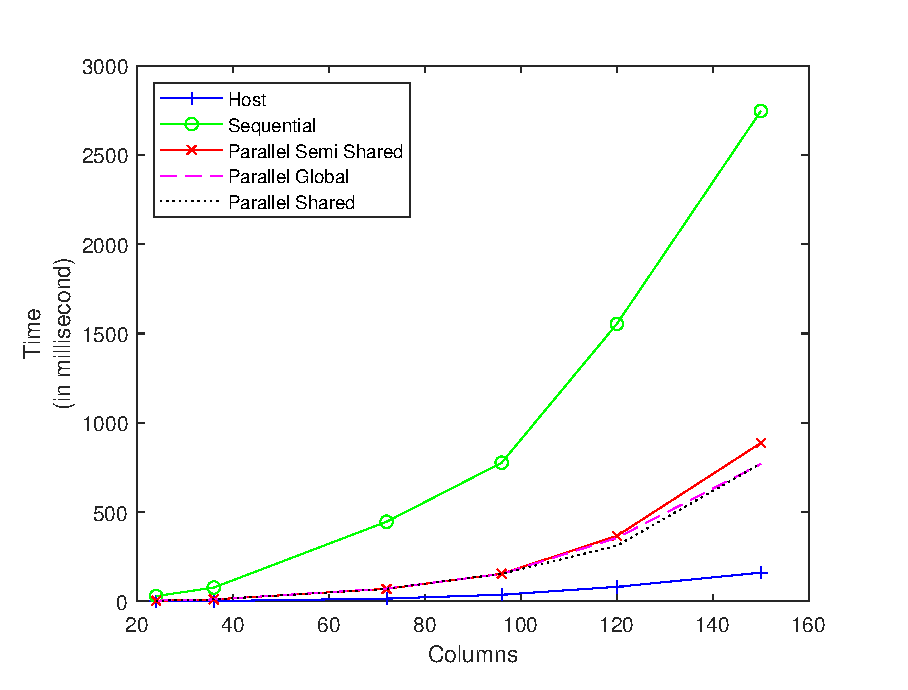
\includegraphics[width=.6\textwidth]{Grafici/ColumnsTime.eps} 
	\label{fig:ColumnsTime}}
	\subfloat[][Dettaglio Columns vs. Time]
	{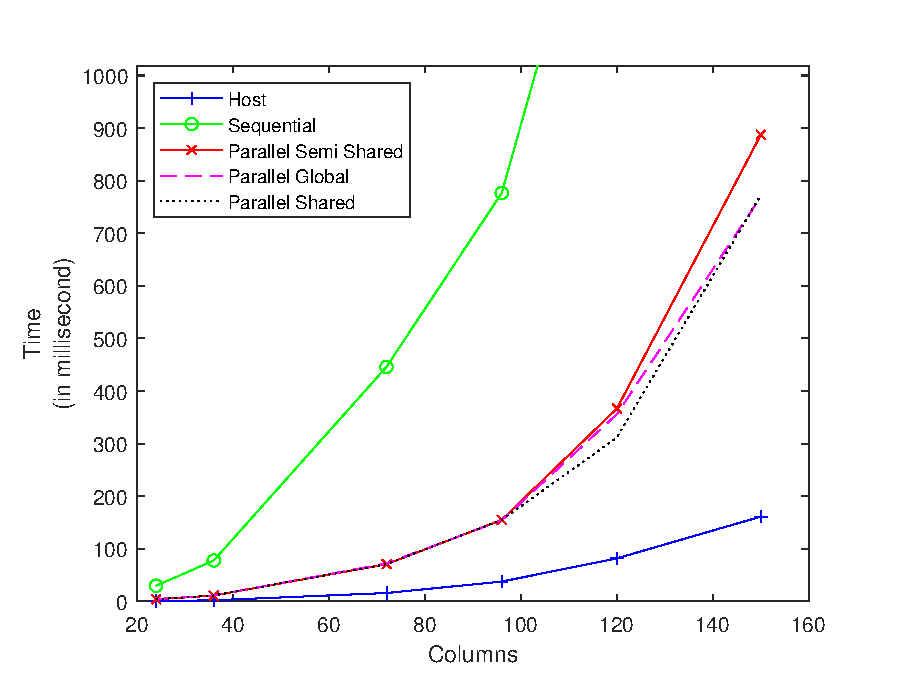
\includegraphics[width=.6\textwidth]{Grafici/ColumnsTime_Zoom.eps} \label{fig:ColumnsTime_Zoom}} \\
	\caption{Confronto Columns vs. Time}
\end{figure}
I grafici che seguono sono stati ottenuti usando lo strumento \textit{nvprof} che consente di raccogliere e visualizzare i dati di profiling dalla riga di comando. \textit{nvprof} consente la raccolta di una sequenza temporale di attività correlate a CUDA su CPU e GPU, tra cui l'esecuzione del kernel, trasferimenti di memoria e chiamate ad API CUDA ed eventi. Le opzioni di profiling vengono fornite a nvprof tramite le opzioni della riga di comando. Nei grafici di sinistra si possono notare le chiamate alle API CUDA, mentre in quelli di destra le prestazioni dei kernel. 

Sull'asse delle ordinate, la misura presa in considerazione è la percentuale di tempo sul totale del programma eseguito sul device. Sull'asse delle ascisse viene riportata la grandezza della matrice, in relazione al numero delle colonne. I grafici presentati sono divisi per tipo di algoritmo preso in considerazione.

Nei grafici~\ref{fig:API_Profiling_Sequential} e~\ref{fig:Kernel_Profiling_Sequential} vengono mostrate le prestazioni dell'algoritmo sequenziale. Nella figura~\ref{fig:API_Profiling_Sequential} si nota che per la matrice con 24 colonne le funzioni che occupano più tempo in percentuale sono \textit{cudaEventCreate} ($49\%$), \textit{cudaDeviceReset} ($23\%$), \textit{cudaLaunch} ($11\%$) e \textit{cudaMemcpy} ($11\%$), mentre per la matrice con 150 colonne sono \textit{cudaLaunch} ($82\%$) e \textit{cudaMemcpy} ($9\%$). La funzione \textit{cudaDeviceReset} distrugge tutte le allocazioni fatte e ripristina lo stato sul device, \textit{cudaLaunch} lancia una funzione del dispositivo. L'aumento della percentuale di tempo relativa a \textit{cudaLaunch} con l'aumentare della dimensione della matrice è conseguenza del fatto che il kernel \textit{rotate} viene richiamato $n(n-1)/2$ volte, dove $n$ è il numero di colonne, come spiegato nel capitolo~\ref{sec:Sequential} e come si può vedere nel codice~\ref{code:sequential_loop}. Il numero di volte con cui viene chiamata la funzione sul device ha andamento quadratico con l'aumentare delle colonne.

Il kernel che impiega più tempo, come si può vedere nella figura~\ref{fig:Kernel_Profiling_Sequential}, è \textit{rotate} per una percentuale di tempo maggiore del $99\%$.
\begin{figure}[H]
	\centering
	\subfloat[][Profiling delle API CUDA \\dell'algoritmo sequenziale]
	{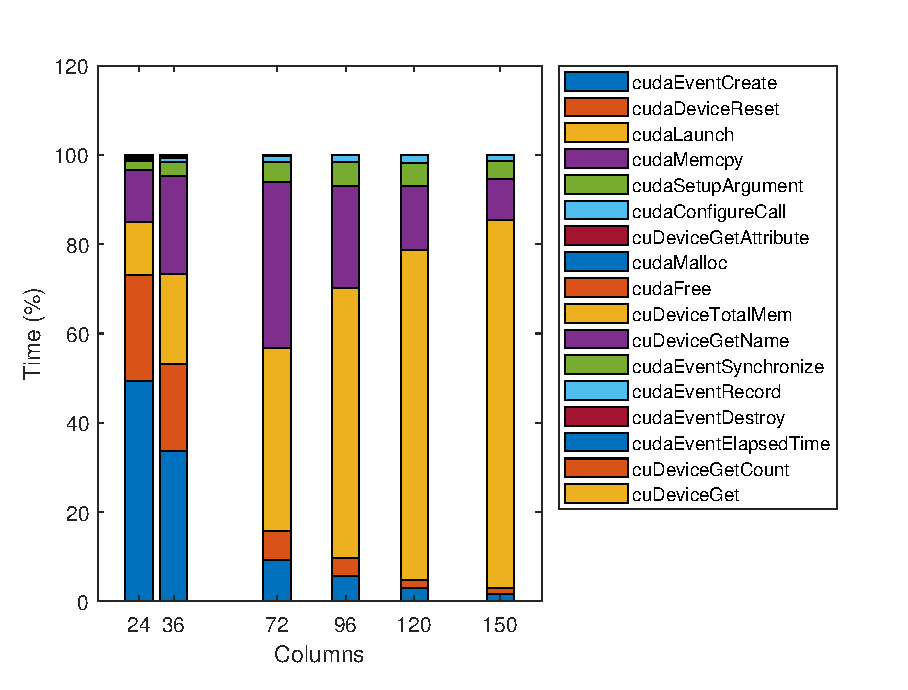
\includegraphics[width=.6\textwidth]{Grafici/API_Profiling_Sequential.eps} \label{fig:API_Profiling_Sequential}}
	\subfloat[][Profiling dei kernel \\dell'algoritmo sequenziale]
	{\includegraphics[width=.6\textwidth]{Grafici/Kernel_Profiling_Sequential.eps} \label{fig:Kernel_Profiling_Sequential}} \\
	\caption{Prestazioni algoritmo sequenziale}
\end{figure}

Nei grafici~\ref{fig:API_Profiling_Parallel_Global} e~\ref{fig:Kernel_Profiling_Parallel_Global} vengono mostrate le prestazioni dell'algoritmo parallel con la matrice \textit{B} salvata nella memoria globale. Come mostrato in figura~\ref{fig:API_Profiling_Parallel_Global}, le funzioni che richiedono più tempo per la matrice più piccola sono \textit{cudaEventCreate} ($58\%$), \textit{cudaDeviceReset} ($35\%$), \textit{cudaMemcpy} ($2\%$) e \textit{cudaLaunch} ($2\%$). Per la matrice più grande sono invece \textit{cudaMemcpy} ($88\%$), \textit{cudaEventCreate} ($5\%$), \textit{cudaDeviceReset} ($3\%$) e \textit{cudaLaunch} ($2\%$). Con l'aumentare della dimensione della matrice la funzione \textit{cudaMemcpy} ($88\%$) predomina dal punto di vista temporale perché occorre fare più copie dalla memoria dell'host a quella del device, e viceversa, della variabile \textit{host\_exit\_flag} come mostrato nel codice~\ref{code:parallel_loop}. 

Il kernel che impiega più tempo in percentuale è \textit{round} con l'$85\%$ per la matrice più piccola e il $96\%$ per quella più grande, mentre \textit{scheduling} impiega rispettivamente il $13\%$ e il $3\%$.

\begin{figure}[H]
	\centering
	\subfloat[][Profiling delle API CUDA \\dell'algoritmo parallelo global]
	{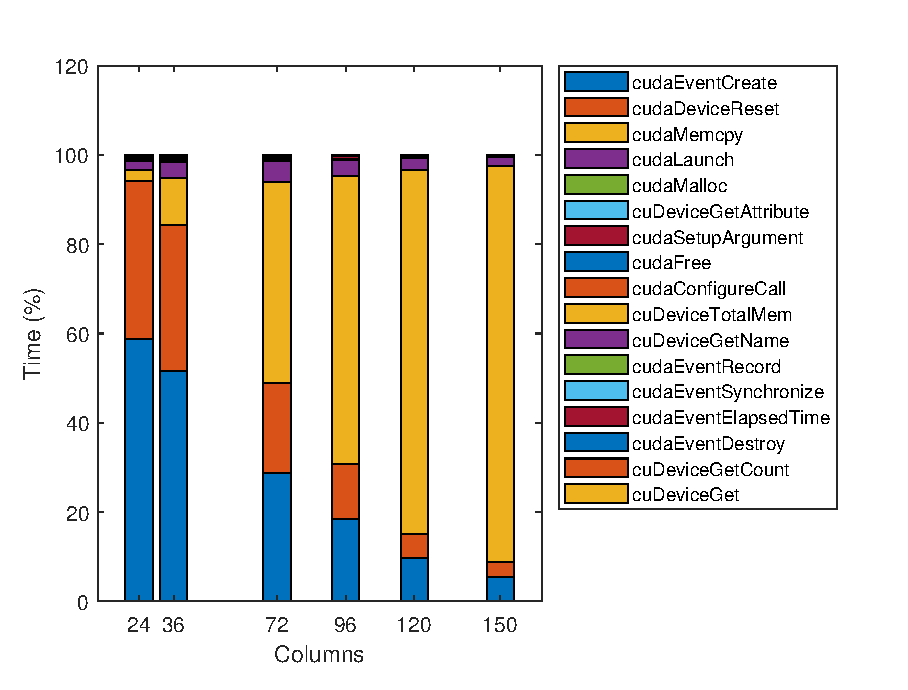
\includegraphics[width=.6\textwidth]{Grafici/API_Profiling_Parallel_Global.eps} \label{fig:API_Profiling_Parallel_Global}}
	\subfloat[][Profiling dei kernel \\dell'algoritmo parallelo global]
	{\includegraphics[width=.6\textwidth]{Grafici/Kernel_Profiling_Parallel_Global.eps} \label{fig:Kernel_Profiling_Parallel_Global}} \\
	\caption{Prestazioni dell'algoritmo parallelo global}
\end{figure}

Nei grafici~\ref{fig:API_Profiling_Parallel_Semi_Shared} e~\ref{fig:Kernel_Profiling_Parallel_Semi_Shared} vengono mostrate le prestazioni dell'algoritmo parallel con la matrice \textit{B} salvata nella memoria globale e con l'uso delle variabili all'interno del kernel salvate nella shared.

Le funzioni che impiegano più tempo per la matrice più piccola sono \textit{cudaEventCreate} ($56\%$), \textit{cudaDeviceReset} ($38\%$), \textit{cudaMemcpy} ($2\%$) e \textit{cudaLaunch} ($2\%$). Per la matrice più grande sono invece \textit{cudaMemcpy} ($89\%$), \textit{cudaEventCreate} ($4\%$), \textit{cudaDeviceReset} ($3\%$) e \textit{cudaLaunch} ($2\%$). 

Il kernel che impiega più tempo in percentuale è \textit{round} con l'$85\%$ per la matrice più piccola e il $96\%$ per quella più grande, mentre \textit{scheduling} impiega rispettivamente il $13\%$ e il $3\%$.

I risultati sono simili a quelli precedentemente descritti: la variazione più importante è nel tempo di esecuzione, mostrata nel grafico~\ref{fig:ColumnsTime_Zoom}, e non nella percentuale di tempo impiegata.

\begin{figure}[H]
	\centering
	\subfloat[][Profiling delle API CUDA \\dell'algoritmo parallelo semi-shared]
	{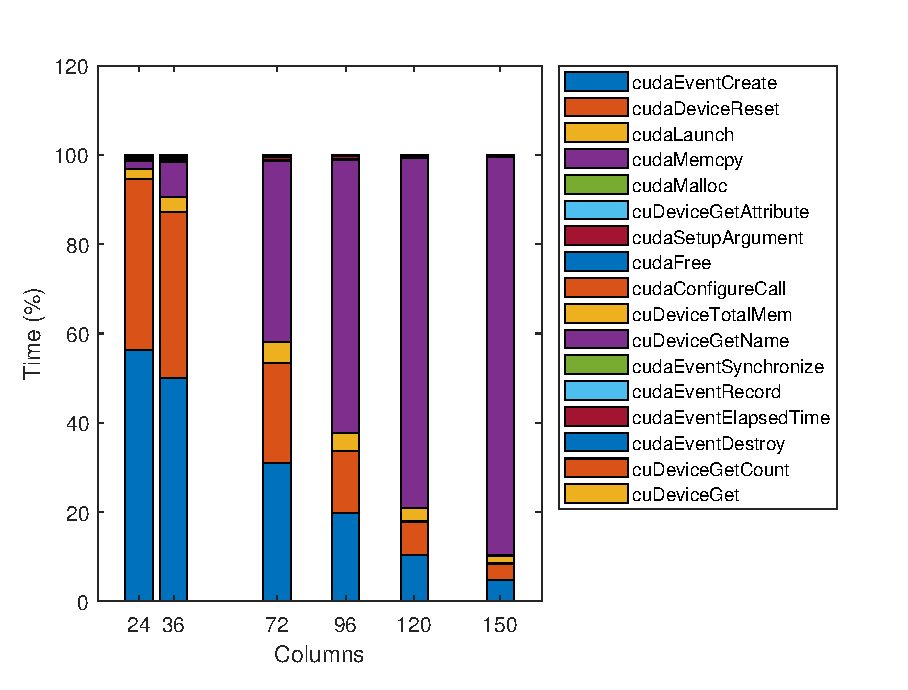
\includegraphics[width=.6\textwidth]{Grafici/API_Profiling_Parallel_Semi_Shared.eps} \label{fig:API_Profiling_Parallel_Semi_Shared}}
	\subfloat[][Profiling dei kernel \\dell'algoritmo parallelo semi-shared]
	{\includegraphics[width=.6\textwidth]{Grafici/Kernel_Profiling_Parallel_Semi_Shared.eps} \label{fig:Kernel_Profiling_Parallel_Semi_Shared}} \\
	\caption{Prestazioni dell'algoritmo parallelo semi-shared}
\end{figure}

Nei grafici~\ref{fig:API_Profiling_Parallel_Shared} e~\ref{fig:Kernel_Profiling_Parallel_Shared} vengono mostrate le prestazioni dell'algoritmo parallel con la matrice \textit{B} e le variabili usate nel kernel salvate nella shared memory.

Anche in questo caso i risultati sono simili a quelli precedentemente illustrati. L'uso della memoria shared per allocare il vettore diminuisce il tempo per completare il kernel \textit{round}, ma non la percentuale di tempo richiesta dalle singole funzioni.

\begin{figure}[H]
	\centering
	\subfloat[][Profiling delle API CUDA \\dell'algoritmo parallelo shared]
	{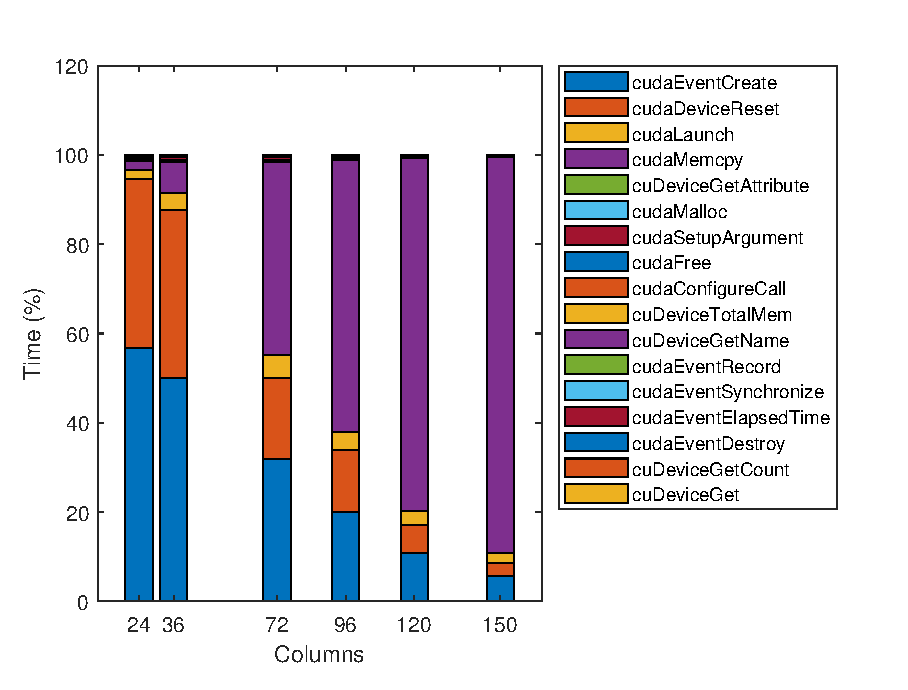
\includegraphics[width=.6\textwidth]{Grafici/API_Profiling_Parallel_Shared.eps} \label{fig:API_Profiling_Parallel_Shared}}
	\subfloat[][Profiling dei kernel \\dell'algoritmo parallelo shared]
	{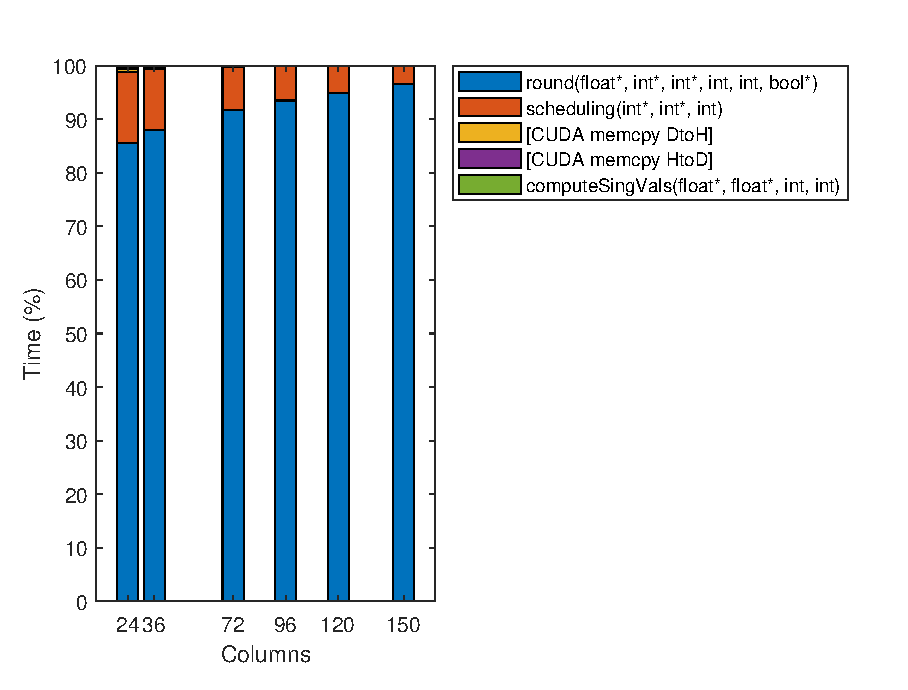
\includegraphics[width=.6\textwidth]{Grafici/Kernel_Profiling_Parallel_Shared.eps} \label{fig:Kernel_Profiling_Parallel_Shared}} \\
	\caption{Prestazioni dell'algoritmo parallelo semi-shared}
\end{figure}


\newpage
\section{Conclusioni}
The CUDA programming model has an inherent design trait that complicates the implementation of \textit{round}. In short, it is impossible to synchronize the execution and global memory transactions of threads in different thread blocks within a running kernel. Without loss of generality, for \textit{round} this means that at the end of a set when thread block b1 writes its orthogonalized columns back to global memory, there is no way to guarantee that thread block b2 will see and read in either of the updated columns at the start of the next set.

In practice, the only way for threads in different thread blocks to synchronize and share data is to relaunch the kernel after each thread block has written its initial results to global memory. This restricts the scope of \textit{round} and forces the host to launch the kernel once per set. This results in the following undesirable consequences:
\begin{itemize}
	\item For every run of \textit{round}, each thread block must read the matrix columns from global	memory into shared memory or only from global memory in base of the implemented algorithm. Since the contents of shared memory are transient, this guarantees that each thread block on every set pays the penalty for reading four column vectors from global memory.
	
	In contrast, if synchronization across thread blocks were possible, it is possible a more intelligent column pair partitioning scheme could be devised. Ideally, such a scheme would minimize the number of global	memory reads a thread block requires at the start of a new set.
	\item Convergence testing must be done on the host. This requires a counter to be stored in global memory that is incremented for each thread block whose column pair is already sufficiently orthogonal. The host then needs to read this value at the end of each set to determine if it needs to continue calling \textit{round}. 
	
	Since the host must read memory from the device after every set, this has the effect of implicitly synchronizing the host with the device after every invocation of \textit{round}. This effectively reduces, if not eliminates,	possibilities for concurrent kernel execution, which in turn limits total throughput.
\end{itemize}

The runtime performance shown in~\ref{sec:Performace} for the implementation of the approach given above was measured on a laptop equipped with an Intel i7-3630 QM 2.40 GHz CPU, 8GB of RAM, and the aforementioned Geforce GTX 610M.

In principle, an SVD based on the one-sided Jacobi method can be adapted to exploit readily available devices with massively parallel capabilities. With it, it is possible to achieve a high degree of thread-level parallelism that is on the order of the number of elements in the matrix.

However, core characteristics of both the programming model and hardware architecture of NVIDIA GPUs make the above approach a bit of a mismatch for them in practice. Most notably a lack of grid-level thread synchronization forces the orthogonalization process to be spread out over multiple kernel invocations. Consequently, the host is forced to synchronize with the device after each set, and the device is unable reduce global memory transactions between sets through caching of data in shared memory. Both of these result in additional overhead that ultimately limits the ability to fully exploit the compute capabilities of the GPU.

Another approach for the SVD is presented in~\cite{Boukaram:SVD}. It's very important when we can no longer store the entire matrix in shared memory, we have to operate on the
matrix in the slower global memory. Instead of repeatedly reading and updating the columns one at a time, block algorithms can operate with blocks of columns.

There are two global memory block Jacobi algorithms that differ only in the way block columns are orthogonalized and there is a comparison of their performance with parallel streamed calls to the cuSOLVER 8 library routines. Our Jetson GPU cannot use this library because we are using CUDA 6.5 and it has a 3.2 compute capability. 

For further work it's recommended to perform the algorithms described with a high-performance GPU that can use cuSOLVER libraries and with a $\geq 3.5$ compute capability: this allows the programmer to increase the parallelism using kernels that are invoking other kernels.

\newpage

\nocite{*}
%Il comando \printbibliography produce la sezione bibliografica con relativi
%titolo e testatina. Per mandarne il relativo titolo nell’indice generale si
%usa l’istruzione:
\printbibliography

\end{document} 